\section*{Комментарии и ссылки}

\subsubsection*{Ангел и Дьявол Конвея}

Недавний обзор этой увлекательной головоломки содержится в очень симпатичной коллекции под редакцией Ричарда Новаковского.\footnote{\emph{Games of No Chance.} Edited by Richard Nowakowski, Cambridge University Press, Cambridge, 1996. \href{http://library.msri.org/books/Book29/}{\url{library.msri.org/books/Book29/}}.} 

Элвин Берлекэмп показал, что если Ангел обладает «силой 1», то есть может делать только одиночные ходы короля, то Дьявол побеждает.
Может оказаться, что Дьявол побеждает независимо от силы Ангела; 
однако, похоже на то, что силы 2 достаточно для того, чтобы Ангел выжил.

Ангел силы 1000 должен быть в состоянии выжить, но как сам изобретатель головоломки говорит в своей статье, на путях к решению возникают помехи.
Одна из них заключается в том, что Дьявол не может ошибиться;
то есть независимо от того, какую клетку он уничтожит, полученная конфигурация станет для него лучше, чем начальная.
Другая заключается в том, что Дьявол, кажется, имеет ответ на любую простую стратегию «потенциальной функции», которой мог бы воспользоваться Ангел;
то есть, стратегия, которая говорит ему, куда ходить в зависимости от того, какие клетки уничтожены. 

Кроме того, если Ангел имеет какие-то, казалось бы, лёгкие недостатки вроде того, что ему запрещено ступать на клетку в далее чем на $10^{99}$ клеток к югу от клетки на которой он уже побывал, то Дьявол побеждает.

Сам Конвей похоже верит в Ангела, об этом свидетельствует то, что он предлагает приз в тысячу долларов за доказательство того, что Дьявол побеждает, и только сто за стратегию для достаточно сильного Ангела.

[Со времени публикации английского оригинала этой книги, задача была независимо решена, как минимум, 4 раза.
Решения Оддвара Клостера%
\footnote{
O. Kloster, 
``A solution to the angel problem''.
\emph{Theoret. Comput. Sci.} 389 (2007), no. 1-2, 152--161.}
и Андре Мате%
\footnote{
A. Máthé, 
``The angel of power 2 wins''. 
\emph{Combin. Probab. Comput.} 16 (2007), no. 3, 363–374.}
работают для ангела силы 2.
Решение Брайна Боудича%
\footnote{B. H. Bowditch, ``The angel game in the plane''. \emph{Combin. Probab. Comput.} 16 (2007), no. 3, 345--362.}
работает для ангела силы 4.
Решения Питера Гакса%
\footnote{G. Peter, \emph{The angel wins.} \href{https://www.cs.bu.edu/~gacs/papers/angel.pdf}{\url{www.cs.bu.edu/~gacs/}}.}
работает для ангела много большей силы.]

\subsubsection*{$\bm{3x+1}$ дилемма}

Эта головоломка известна так же как гипотеза Коллатца, Сиракузская задача, задача Какутани, алгоритм Хасса и гипотеза Улама.
Мало что известно об её источнике, только, что 1 июля 1932 года, студент Гамбургского университета по имени Лотар Коллатц записал похожую задачу в свою тетрадь, но задача, известная теперь, кажется, стала популярна только в 1950-е годы.

Джефф Лагариас из лабораторий AT\&T написал о ней очень хороший обзор.\footnote{J. Lagarias, ``The 3x+1 Problem and its Generalizations''. \emph{Amer. Math. Monthly}, Vol. 92 (1985), 3--23,%\href{http://www.cecm.sfu.ca/organics/papers/lagarias/}{\url{www.cecm.sfu.ca/organics/papers/lagarias/}}.
}

Лагариас указывает на то, что эта головоломка упоминалась как часть заговора с целью замедлить математические исследования в США.
Пусть это послужит предупреждением!

\subsubsection*{Самая длинная общая подпоследовательность}

Эта задача известна, как минимум, с 30-х годов;
она упоминается в диссертации В. Данчика 1974 года, защищённой в Уорикском университете.
Майкл Стил (Пенсильванский университет) сформулировал гипотезу, что $C_{1/2} = 2/(1+\sqrt{2})\approx 0{,}828427$.
Вацлав Хватал и Давид Санкофф показали, что $0{,}773911 < C_{1/2} < 0{,}837623$, и это дало основание предполагать, что число Стила великовато;
в конце концов, Джордж Люкер (Калифорнийский университет в Ирвайне) добил гипотезу, доказав, что $0{,}7880 \z< C_{1/2} \z< 0{,}8263$.\footnote{
G. Lueker, 
``Improved bounds on the average length of longest common subsequences''. \emph{Proceedings of the Fourteenth Annual ACM-SIAM Symposium on Discrete Algorithms} (Baltimore, MD, 2003), 130–131.}

Существование $C_p$ легко следует из субаддитивности,\footnote{см., например, R. Durrett, \textit{Probability: Theory and Examples,} Wadsworth, 1991, Section 6.6.} но это не позволяет вычислить саму константу.
Вот ещё подобный пример: Бела Боллобаш и я доказали существование числа $K_d$ такого, что самая длинная координатно-возрастающая цепь среди $n$ случайных точек в $d$-пространстве имеет средний размер равный $K_d\cdot n^{1/d}$.
Мы знаем, что $K_1=1$, $K_2=2$ и $\lim_{d\to\infty} K_d=e$, но не знаем, чему равно $K_3$.

Если менять вероятность $p$, то, конечно же, $C_p>p$ при $p \z> 1/2$, так как можно смотреть только на подпоследовательности, состоящие из одних единиц.
Таким образом, $C_p\to 1$ при $p\to 1$, и это даёт основание предполагать, что $C_p$ минимально при $p=1/2$.
Чтобы это доказать, необязательно знать точные значения $C_p$,
но, как это сделать, пока никто не знает.

\subsubsection*{Квадратура озера}

Хорошее обсуждение этой головоломки дано на «Геометрической свалке» Давида Эпштейна.%
\footnote{\href{http://www.ics.uci.edu/~eppstein/junkyard/jordan-square.html}{\url{www.ics.uci.edu/~eppstein/junkyard/jordan-square.html}}}
Похоже, что есть доказательства того, что квадрат можно вписать во все достаточно гладкие замкнутые плоские кривые.%
\footnote{Например, W. Stromquist, ``Inscribed Squares and Square-Like Quadrilaterals in Closed Curves''. \emph{Mathematika}, Vol. 36 (1989), No. 2, 187--197.}
Тем не менее в общем случае гипотеза остаётся открытой уже более 90 лет.%
\footnote{V. Klee, S, Wagon, \emph{Old and New Unsolved Problems in Plane Geometry and Number Theory.} MAA, 1991.}

\medskip

Как-то неловко признать, что математики не способны вписать квадрат в любую замкнутую плоскую кривую.

\subsubsection*{Одинокий бегун}

{

\sloppy

Эта замечательная гипотеза, была, по-видимому, выдвинута Йоргом Виллсом.%
\footnote{J. M. Wills, ``Zwei Satze uber Inhornogene Diophantische Approximation von Irrationalzahlen''. \emph{Monatsch. Math.}, Vol. 71 (1967), 263--269.}
В 1973 году её независимо сформулировал Томас Кьюсик.
В 1984 году он вместе с Карлом Померансом доказал гипотезу для не более, чем пяти бегунов.
Том Бохман, Рон Хольцман и Дэн Клейтман (те самые, что из ящиков и подъящиков) доказали её для шести,%
\footnote{T. Bohman, R. Holzman, D. Kleitman,
``Six lonely runners''.
\emph{Electron. J. Combin.} 8 (2001), no. 2.
%\href{https://www.combinatorics.org/ojs/index.php/eljc/article/view/v8i2r3/pdf}{\url{www.combinatorics.org/ojs/index.php/eljc/article/view/v8i2r3/pdf}}
}
есть также более короткое доказательство Джерома Рено.%
\footnote{J. Renault, ``View-obstruction: a shorter proof for 6 lonely runners''. \emph{Discrete Math.} 287 (2004), no. 1-3, 93--101.}

}

\medskip

Название головоломки предложил Луис Годин из Университета Саймона Фрейзера.

Головоломка носит численно-теоретический характер;
можно доказать, что достаточно рассмотреть только случай целых скоростей.

\subsubsection*{Сортировка шаров}

Эта любопытная задачка возникла в лаборатории Bellcore (ныне iconectiv) при статистических исследованиях предпочтений заказов.
Я работал над ней с коллегами Майклом Литтманом (ныне в Рутгерсе) и Грэмом Бригиттом (Лондонская школа экономики).
Задача обобщается не только на $k$-шарные корзинки, но и на корзинки с различным числом шаров.
Мы сосредоточимся только на двухшарном случае.

\medskip

Если бы корзинки были одношарные, то задача превратилась бы в простое упражнение.
В этом случае для сортировки обратного порядка требуется $\binom{n}{2}$ перекладываний.
Для того чтобы это увидеть заметим, что в начальный момент все пары шаров находятся в обратном порядке, и одно перекладывание исправляет только одну пару.
Это также влечёт, что если не делать глупостей (а именно, не менять шары, которые уже находились в правильном порядке), то потребуется ровно $\binom{n}{2}$ перекладываний.
Более того, независимо от начальной конфигурации $\binom{n}{2}$ перекладываний достаточно; как и следовало ожидать обратный порядок является наихудшим.

\medskip

Похоже, что те же рассуждения работают и с двухшарными корзинками.
Можно думать, что у нас по $n$ шаров двух цветов, красных и зелёных, и шары каждого цвета пронумерованы от $1$ до~$n$.
Если сортировать каждый цвет по отдельности, то закончим за $2\binom{n}{2}$ перекладываний.
Наверняка $2\binom{n}{2}$ шагов необходимо, верно?

А вот и нет!
В случае $n = 5$ (посмотрите на приведённую ниже диаграмму)
\begin{figure}[h!]
\centering
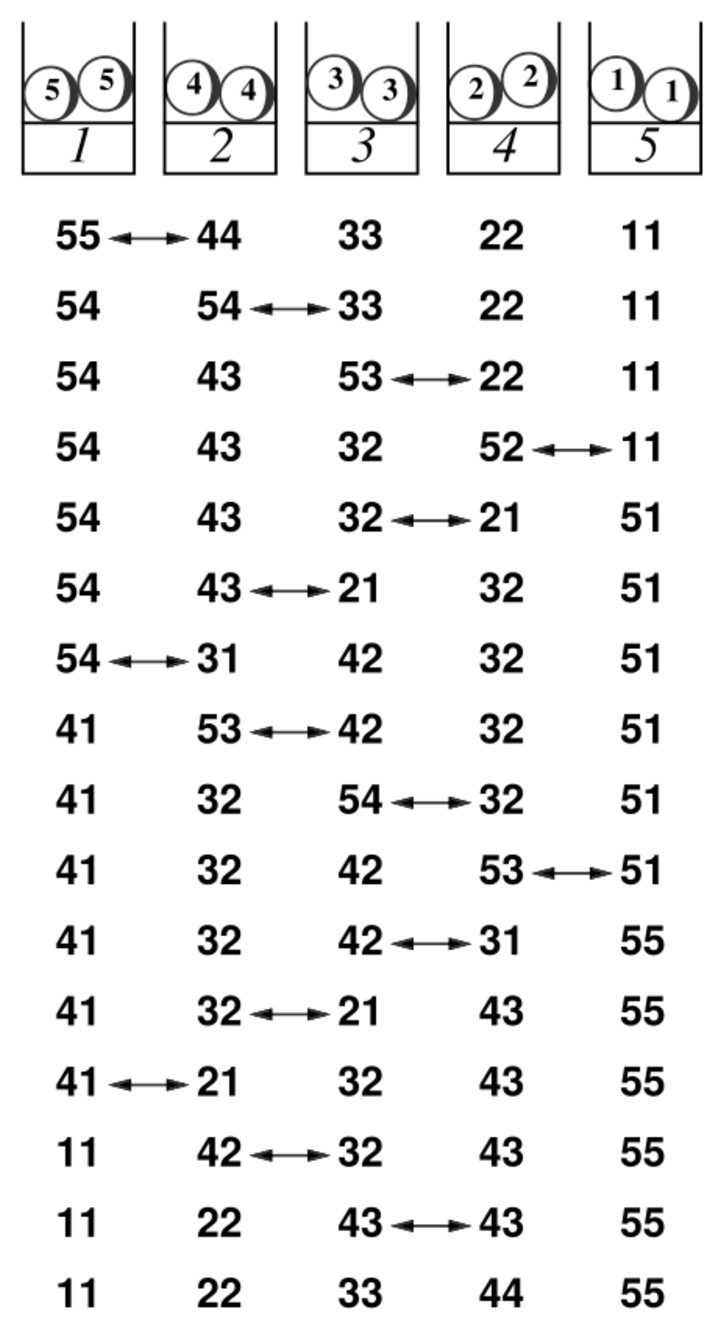
\includegraphics[scale=0.5]{Figs/UnsolvedPuzzles/5bin}
\end{figure}
волшебным образом шары упорядочились за 15 перекладываний, вместо 20, которые казались необходимыми.

Меньше, чем за 15 перекладываний этого добиться нельзя.
Более того, $\lceil\binom{2n}{2}/3\rceil$ перекладываний необходимо для упорядочивания шаров в $n$ двухшарных корзинках.
Чтобы увидеть это, будем давать одно очко за обгон, то есть за то, что шар с б\'{о}льшим номером прошёл слева направо относительно шара с меньшим номером.
Если обгон проделывается в два приёма, то мы назначаем по пол-очка за то, что шар «поравнялся» и за то, что «ушёл вперёд».
Кроме того заметим, что в процессе любая пара шаров с одинаковыми номерами должна разделиться, а потом сойтись вместе --- накинем ещё по пол-очка за каждое такое перекладывание. 
В процессе сортировки придётся собрать $\binom{2n}2$ очков.

А сколько очков можно заработать за одно перекладывание?
Предположим, что мы поменяли шары с номерами $u$ и $y$ из корзинки с $u$ и $v$, и соседней корзинки с $x$ и $y$.
Мы можем получить одно очко за то, что $u$ обогнал $y$,
по пол-очка за то, что $u$ ушёл вперёд от $v$,
и за то, что $x$ ушёл вперёд от $y$,
а ещё по пол-очка за то, что $u$ поравнялся с $x$, 
и за то, что $v$ поравнялся с $y$.
Получается максимум 3 очка за перекладывание;
отсюда следует обещанная оценка.


Есть ещё хорошие новости.
Как и в случае с одношарными корзинками нетрудно показать, что обратный порядок самый плохой.
То есть, если $f_2(n)$ обозначает минимальное число перекладываний, необходимых для сортировки шаров в $n$ двухшарных корзинках из любой начальной конфигурации, то ровно $f_2(n)$ перекладываний потребуется для сортировки обратного порядка.
Также легко доказать, что если обмен должен быть сделан между $i$-той и $(i+1)$-ой корзинками, то не может быть неправильным перекладывать шар с наибольшим номером в $i$-той корзинке с шаром с наименьшим номером в $(i+1)$-ой корзинке.

Но есть и плохие новости, иначе задача не появилась бы в этом разделе.
Оценка $\lceil\binom{2n}{2}/3\rceil$ не всегда достижима.
Например, она даёт $f_2(6)\ge 21$, но на самом деле перебор, проделанный на компьютере, не нашёл способа провести сортировку шаров в шести двухшарных корзинках менее, чем за 22 шага.
Хуже того, закономерность перекладываний для пяти корзинок, показанная на диаграмме, обычно не оптимальна для большего числа корзинок.

Но всё ещё возможно, что какая-то другая закономерность оптимальна, и, возможно, она даёт красивую формулу для $f_2(n)$.

\subsubsection*{Развёртка многогранника}

Есть основания полагать, что эта головоломка \emph{очень} старая. 
Во всяком случае развёртки многогранников рассматривались уже в книге с длинным заглавием «Руководство к измерению циркулем и линейкой, в плоскостях и целых телах, составленное Альбрехтом Дюрером и напечатанное с соответствующими чертежами в 1525 году на пользу всем любящим искусство».
Если требуется разукрасить поверхность многогранника, то первое, что приходит в голову это разрезать её вдоль рёбер и развернуть на плоскости без перекрытий.

По-видимому, первая точная формулировка этой головоломки дана Г. С. Шепардом из Университета Восточной Англии.%
\footnote{G. C. Shephard, ``Convex Polytopes with Convex Nets''. \emph{Math. Proc. Camb. Phil Soc}, Vol. 78 (1975), 389--403.}
 
Известно, что существуют \emph{не}выпуклые неразвёртываемые многогранники%
\footnote{M. Bern, E. Demaine, D. Eppstein, E. Kuo, A. Mantler, J. Snoeyink, 
``Ununfoldable polyhedra with convex faces''.
\emph{Comput. Geom.} 24 (2003), no. 2, 51-–62.};
также существуют выпуклые многогранники, у которых наряду с честными развёртками, есть развёртки с самоперекрытиями. 
Пара развёрток тетраэдра с перекрытием и без, построенная Макото Намики из Токийского университета, показана ниже.

\begin{figure}[h!]
\centering
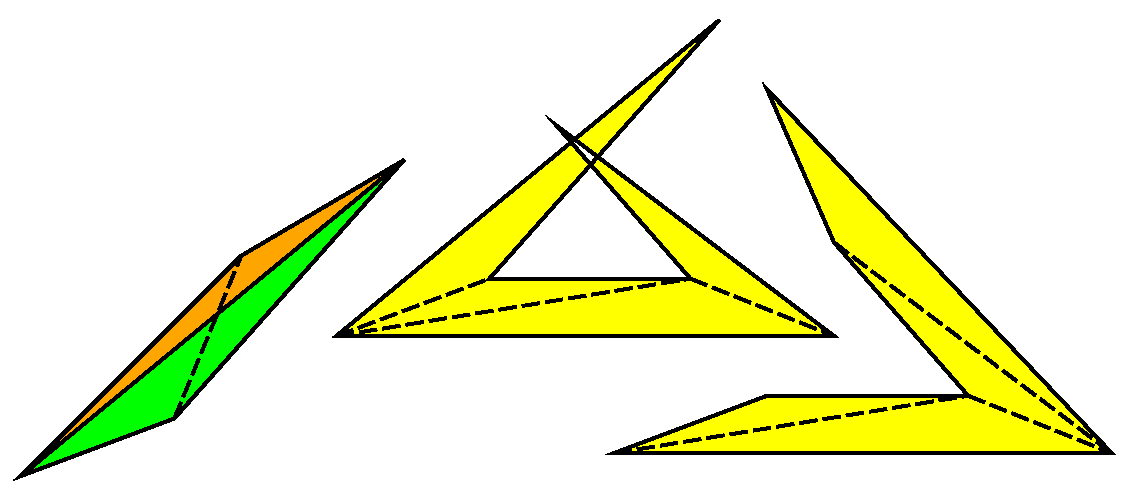
\includegraphics[scale=0.5]{Figs/UnsolvedPuzzles/unfold}
\end{figure}

Между прочим, это покажется интересным --- не по каждой развёртке можно восстановить исходный выпуклый многогранник однозначно. %реф

Обсуждение этой задачи и дополнительные картинки можно найти на домашней странице Комеи Фукуда из Высшей технической школы Цюриха.%
\footnote{\href{https://inf.ethz.ch/personal/fukudak/old/}{\url{inf.ethz.ch/personal/fukudak/old}}}

\subsubsection*{Освещение многоугольника}

В своей книге%
\footnote{J. O'Rourke \emph{Art Gallery Theorems and Algorithms.} Oxford University Press, 1987.}
Джозеф О’Рурк % (Joseph O' Rourke) 
из Смит Колледжа утверждает, что источник этой головоломки неизвестен.
Виктор Кли написал о ней в 1969 году в статье, вышедшей в «American Mathe\-ma\-tical Monthly», которая привлекла большое внимание. 

Если считать, что луч, попавший в вершину поглощается, то можно построить многоугольник, который не освещён из некоторой своей внутренней точки.
Пример, представленный ниже, найден Джоржем Токарским в 1995 году.

\begin{figure}[h!]
\centering
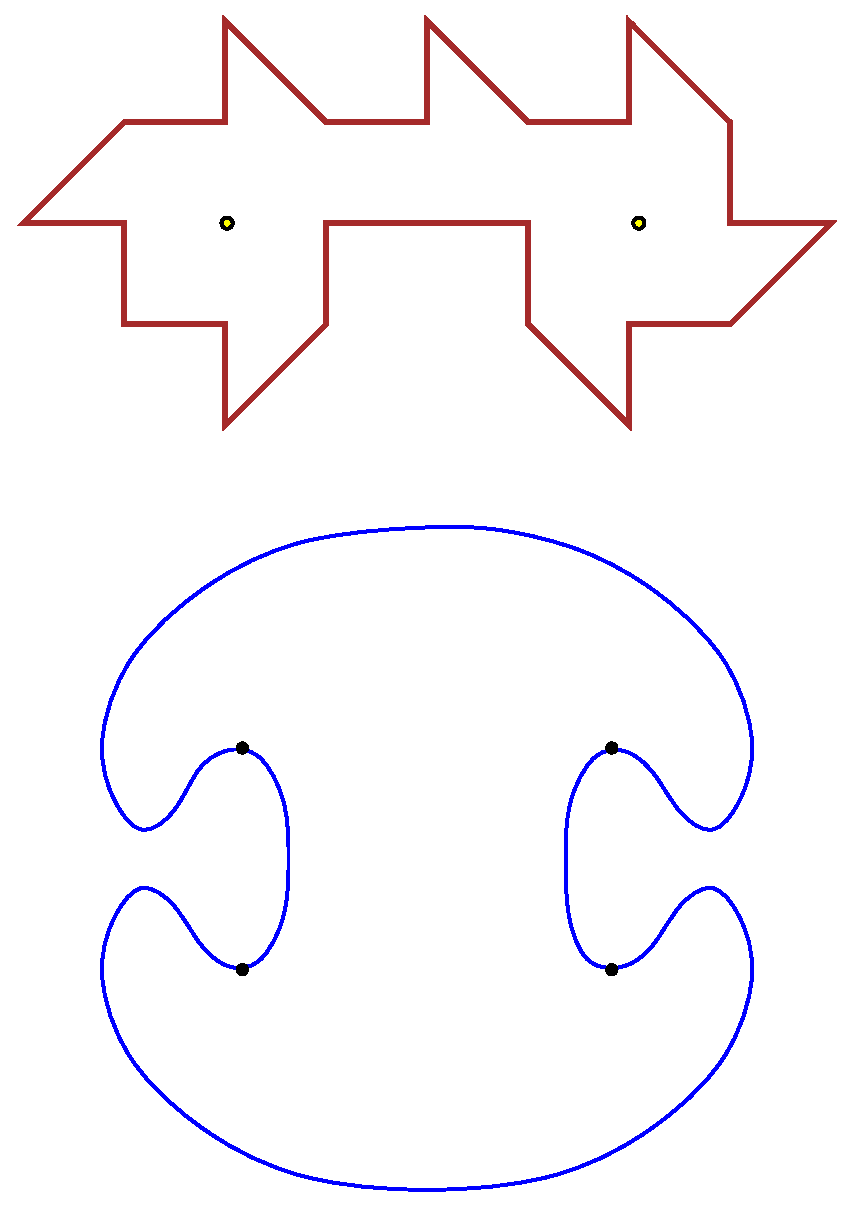
\includegraphics[scale=0.5]{Figs/UnsolvedPuzzles/vision}
\end{figure} 

О’Рурк полагает, что в любом зеркальном многоугольнике $P$ множество внутренних точек, из которых $P$ не может быть освещено, имеет меру 0.
Более того, если вершины заменяются небольшими круглыми дугами, то таких точек вовсе нет.

{\sloppy

Можно сконструировать фигуру, ограниченную гладкой замкнутой кривой, которая не может быть освещена ни из одной своей внутренней точки. 
Такой пример был построен самим Кли (показан здесь), он использует два полуэллипса с фокусами в указанных точках.%
\footnote{Практически идентичный пример приведён ранее в заметке L. Penrose, R. Penrose, ``Puzzles for christmas''. \emph{New Scientist} 25 (1958), 1580--1581.}
Источник света в верхней половине оставляет тёмной левую и правую доли на нижней половине.

}

\begin{figure}[h!]
\centering
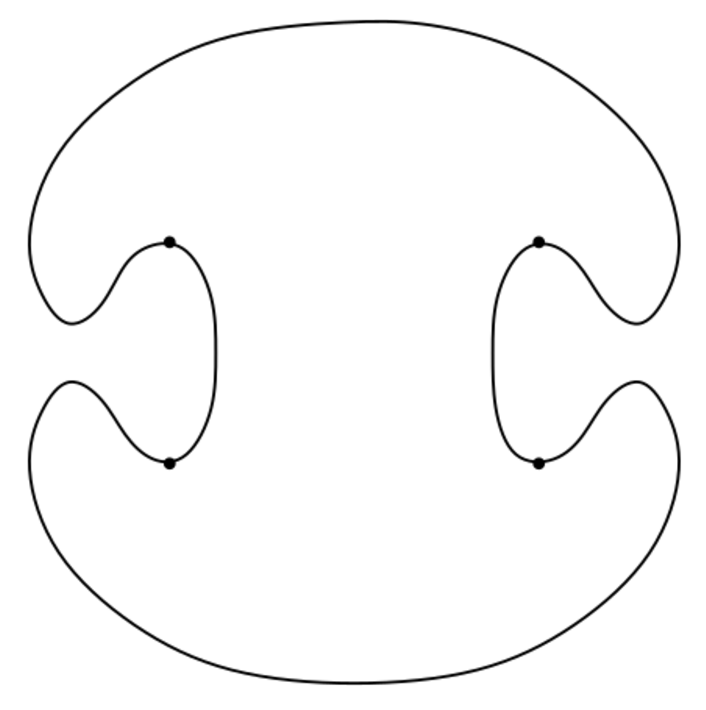
\includegraphics[scale=0.5]{Figs/UnsolvedPuzzles/klee}
\end{figure} 

Есть довольно много других интригующих вопросов про зеркала.
Например, может ли конечный набор разделённых сегментных зеркал захватывать свет от источника?
А что насчёт зеркал в форме дуг окружностей?
Это и многое другое можно найти на слайдах замечательного доклада О’Рурка.%
\footnote{J. O'Rourke, ``Unsolved Problems in Visibility,''
%???--->{\url{archive.dimacs.rutgers.edu/dci/2001/Visibility.ppt}}.
}

\subsubsection*{Треклы Конвея}

Эта интригующая гипотеза Конвея относится к 60-м годам.%
\footnote{D. R. Woodall, ``Thrackles and Deadlock''. \emph{Combinatorial Mathematics and its Applications}, Proceedings of a Conference held at the Mathematical Institute, Oxford (1969), 335--348.}
Её можно свести к тому, что два чётных цикла, склеенных по вершине невозможно представить как трекл;
что, конечно, смущает ещё больше.
Лучшая известная мне оценка даёт, что число рёбер не может превышать удвоенное число вершин минус~3.%
\footnote{L. Lovasz, J. Pach, M. Szegedy, ``On Conway's Thrackle Conjecture''. \emph{Discrete and Computational Geometry}, Vol. 18 (1997), 369--376.}

У этой головоломки имеется свой фан-клуб.%
\footnote{\href{http://www.thrackle.org}{\url{www.thrackle.org}}.}

\subsubsection*{Затор}

Эта модель возникала при изучении транспортного потока на пересечении двух широких односторонних улиц.%
\footnote{O. Biham, A. A. Middleton, D. Levine, ``Self Organization and a Dynamical Transition in Traffic Flow Models''. \emph{Phys. Rev. A}, Vol. 46.10 (1992) R6124.}
Странное поведение модели вызвало большой интерес.%
\footnote{Библиографию можно найти по адресу \href{http://cui.unige.ch/spc/Bibliography/traffic.html.}{\url{cui.unige.ch/spc/Bibliography/traffic.html}}.}
Ниже показаны фрагменты конфигураций, свободной и блокированной, каждая из которых похожа на то, что появлялось в экспериментах, проведённых Раисой Де Соуза из Microsoft Research.

\begin{figure}[h!]
\centering
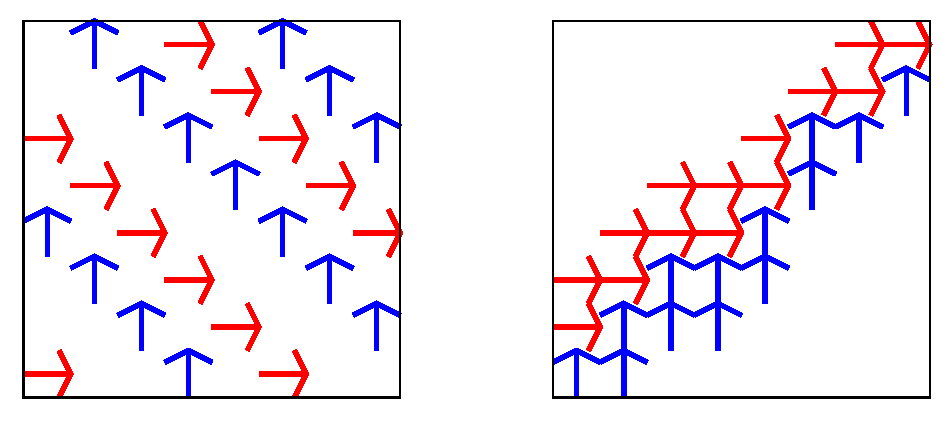
\includegraphics[scale=0.5]{Figs/UnsolvedPuzzles/gridlock}
\end{figure}

Если бы только доказать, что для \emph{некоторых} $p$, пусть даже очень близких $0$ или $1$, поведение на самом деле такое...

[Со времени публикации английского оригинала этой книги случай $p\approx 1$ был решён Омером Энджелом,
Александром Холройдом и Джеймсом Мартином.
\footnote{O. Angel, A. Holroyd, J. Martin, 
``The jammed phase of the Biham--Middleton--Levine traffic model''.
\emph{Electron. Comm. Probab.} 10 (2005), 167--178.}]

\subsubsection*{Гипотеза о средних уровнях}

Эта знаменитая головоломка о гамильтоновом цикле приписывалась в разные времена комбинаторикам: Ивану Гавелю, Клоду Берже, Итало Деджтеру, Палу Эрдёшу, У. Т. Троттеру и Дэвиду Келли.
Вероятно, Гавел был первым.
Вопрос лежит на поверхности, и неудивительно, что он был придуман много раз.
Келли представил головоломку на конференции в Обервольфахе в 1981 году и получил приз (бутылку вина) за самую короткую гипотезу.

%Предупреждение читателю: Эта задачка заразительна. %и действительно, эксперименты привели многих интеллектуальных следователей к мнению, что существует модель, которая будет работать для любого $n$.
%Никто не верит, что предположение ложно.
Роберт Рот (Университет Эмори) провёл несколько компьютерных экспериментов много лет назад, которые говорят о том, что \emph{число} гамильтоновых циклов \emph{очень} быстро растёт по $n$.
То, что это число может достигнуть нуля для некоторых $n$ кажется неправдоподобным, но нет никаких доказательств обратного.

Лучший частичный результат можно найти в диссертации Роберта Джонсона, студента Имре Лидера из Кембриджа.
Джонсон показал, что по мере увеличения $n$ существуют циклы через произвольно высокую долю множеств среднего уровня.

[Со времени публикации английского оригинала этой книги, эту задачу решил Торсен Мюце.%
\footnote{T. Mütze, 
``Proof of the middle levels conjecture''.
\emph{Proc. Lond. Math. Soc.} (3) 112 (2016), no. 4, 677–-713.}]

\subsubsection*{Построение диаграмм Венна}

Эта головоломка, как и предыдущая, о существовании гамильтонова цикла. 
Действительно, для того чтобы добавить новую область к диаграмме Венна необходимо нарисовать замкнутую кривую, которая пройдёт ровно раз через каждую область.
Эту гипотезу придумал ваш автор.%
\footnote{P. Winkler, ``Venn Diagrams: Some Observations and an Open Problem''. \emph{Congressus Numerantium}, Vol. 45 (1984), 267--274.}

Если разрешить пересечения более чем двух кривых, то любая диаграмма допускает продолжение; это доказли Киран Чилакамарри, Петер Хамбургер и Раймонд Пипперт.%
\footnote{K. B. Chilakamarri, P. Hamburger, R. E. Pippert,
``Simple, Reducible Venn Diagrams on Five Curves and Hamiltonian Cycles''. \emph{Geometriae Dedicata}, Vol. 68 (1997), 245--262.}
Двойственную задачу решили Гара Пруессе и Франк Рускей.%
\footnote{
G. Pruesse, F. Ruskey,
``All Simple Venn Diagrams are Hamiltonian''.
\texttt{arXiv:1504.06651 [math.CO]}.
}
Тем не менее изначальная гипотеза остаётся открытой уже 20 лет.

Electronic Journal of Combinatorics поддерживает несколько полезных веб-обзоров, среди которых один о диаграммах Венна, написанный в основном Фрэнком Рукси, специалистом в этой области из Университета Виктории.%
\footnote{F. Ruskey, M. Weston, \emph{A Survey of Venn Diagrams} \href{http://www.combinatorics.org/Surveys/ds5/VennEJC.html}{\url{www.combinatorics.org/Surveys/ds5/VennEJC.html}}.}
Сами диаграммы известны с 1880 года.%
\footnote{J. Venn,
``On the Diagrammatic and Mechanical Representation of Propositions and Reasonings''.
\emph{The London, Edinburgh, and Dublin Philosophical Magazine and Journal of Science}, Vol. 9 (1880),  1--18.}

То, что эти диаграммы изучаются уже 123 года вовсе не даёт иммунитета от элементарных новых идей!
Например, недавно была решена другая гипотеза --- были построены диаграммы Венна с вращательной симметрией любого простого порядка.%
\footnote{J. Griggs, C. E. Killian, C. D. Savage, ``Venn diagrams and symmetric chain decompositions in the Boolean lattice''.
\emph{The electronic journal of combinatorics}, 11(1), (2004)  2.}

\subsubsection*{Стратегия для игры в щёлк}

Игра щёлк была изобретена Дэвидом Гейлом в 1974 году,%
\footnote{D. Gale ``A Curious Nim-Type Game''. \emph{Amer. Math. Monthly }, Vol. 81 (1974), 876--879)}
 название%
\footnote{англ. chomp --- буквально, чавк.}
 ей дал Мартин Гарднер.
Однако эта игра эквивалентна игре, придуманной ранее Фредериком Шухом.%
\footnote{F. Schuh ``Spel van Delers''. \emph{Nieuw Tijdschrifi voor Wiskunde}, Vol. 39 (1952), 299--304.}
В игре Шуха положительное целое число $k$ фиксируется, и игроки по очереди называют делители $k$, которые не кратны уже названным.
Проигравший тот, кому приходится назвать $1$.

Если $k$ имеет вид $p^mq^n$ при простых $p$ и $q$, то все делители имеют вид $p^iq^j$ при $0 \le i \le m$, $0 \le j \le n$.
При этом на пару $(i,j)$ налагаются те же ограничения, что и в игре щёлк на $(m+1)\times(n+1)$-плитке шоколада.
Более того, $d$-мерная плитка шоколада эквивалентна игре Шуха, если выбранное число $k$ имеет ровно $d$ простых делителей.

Рассуждение с кражей стратегии прекрасно работает и для этого обобщения.
Первый игрок должен иметь выигрышную стратегию, поскольку он может передать первый ход второму игроку выбрав «$k$» в начале игры.
Но никто не знает, что это за стратегия.

Авантюрно настроенные ребята задумывались о том, как бы разрешить трансфинитные ординалы в щёлке.
Ещё более общий вариант «ЧУМ игры», где начинают с фиксированного частично упорядоченного множества $P$, из которого два игрока поочерёдно выбирают элементы.
При этом ни один из игроков не может взять элемент, который больше или равен любому из ранее выбранных, проигрывает, сделавший последний ход.
На момент написания этой книги, последняя хорошая теорема о ЧУМ играх была доказана Стивеном Дж. Бирнсом, старшеклассником из Уэст-Рокбери, Массачусетс.
В 2002 году за эту теорему он получил стипендию в размере ста тысяч долларов на конкурсе Siemens Westinghouse.

\subsubsection*{Все дороги ведут в Рим}

Эта головоломка появилась в серьёзной статье.%
\footnote{R. L. Adler, L. W. Goodwyn, B. Weiss, ``Equivalence of Topological Markov Shifts''. \emph{Israel J. Math}, Vol. 27 (1977), 49--63.}
После того как дороги раскрашены, можно думать про К и С как про операции на множествах вершин.
То есть К$(S)$ --- множество всех вершин, доступных по красному ребру от некоторой вершины из $S$, и С$(S)$ аналогично.
Тогда гипотеза утверждает, что для некоторой окраски существует конечная композиция из К и С, которая сворачивает множество всех вершин в одну.

На рисунке показаны две раскраски полного орграфа с тремя вершинами.
Первую невозможно свернуть, так как $|\text{К}(S)|\z=|\text{С}(S)|\z=|S|$ для любого $S$.
Вторую раскраску сворачивает КС или СК.

\begin{figure}[h!]
\centering
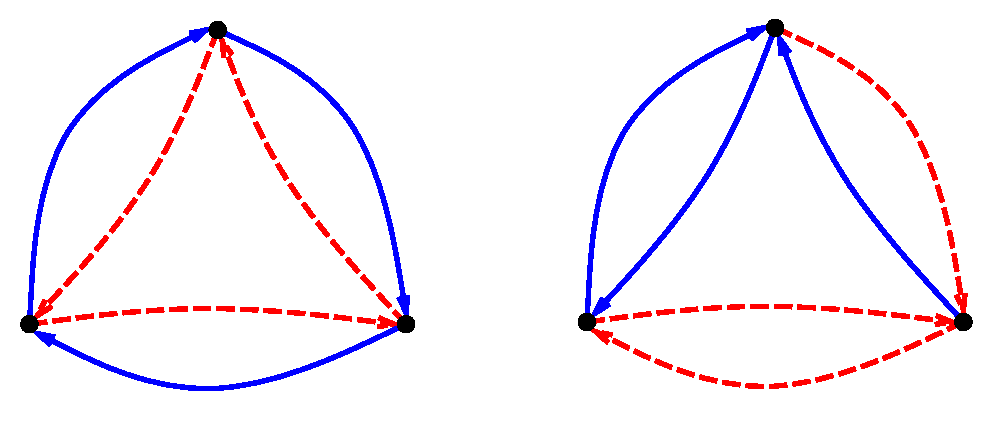
\includegraphics[scale=0.5]{Figs/UnsolvedPuzzles/roads}
\end{figure}

Гипотеза доказана для некоторых классов графов, например, если в каждый город заходят ровно две дороги, и число городов нечётно.%
\footnote{J. Friedman, ``On the Road Coloring Problem''. \emph{Proc A.M.S.}, Vol. 110, No. 4 (December 1990), 1133--1135}

[Со времени публикации английского оригинала этой книги, эту задачу решил Абрам Трахтман.%
\footnote{A. N. Trahtman, 
``The road coloring problem''.
\emph{Israel J. Math.} 172 (2009), 51--60.}]


\subsubsection*{Круги в круге}

Эта прекрасная гипотеза сформулирована Александром Сойфером из Университета Колорадо.
Она и родственные ей гипотезы стали предметом дюжины статей в журнале Geocombinatorics.
Известно, например, что квадраты общей площадью 1 могут быть упакованы в квадрат общей площадью 2.
Обобщение на высшие размерности было предложено, в частности, вашим автором.
Случай двух шаров, каждый объёма $\tfrac12$, показывает, что $2^{d-1}$ нельзя улучшить.

\subsubsection*{Гипотеза Франкла}

Наша последняя головоломка о простейших математических объектах --- конечных множествах.
Увы, даже они способны привести в ступор.

Эта печально известная гипотеза, похоже, возникла впервые в 1970-х годах в творчестве Петера Франкла, венгерского математика, живущего в Японии (и являющегося там известной телевизионной фигурой).
С тех пор она сводит комбинаториков с ума. 
На сегодня им даже неизвестно, существует ли элемент, покрытый какой-либо фиксированной долей множеств из семейства.

Очень хитрое доказательство Э. Кнолла, приведённое в статье Петра Вуйчика,%
\footnote{P. W\'{o}jcik, ``Union-Closed Families of Sets''. \emph{Discrete Math.}, Vol. 199 (1999), 173--182.}
показывает, что существует элемент, содержащийся, по крайней мере, в $N/\log_2 N$ множествах, где $N$ --- размер семейства.

Недавний прогресс по головоломке был сделан Дэвидом Реймером из колледжа Нью-Джерси.%
\footnote{D. Reimer, ``An average set size theorem''. \emph{Combinatorics, Probability and Computing.} Vol. 12 (2003), 89--93.}
Реймер показал, что средний размер множества в семействе, замкнутом по объединению, составляет, по меньшей мере, $\tfrac12\log_2N$ (это было недоказанное следствие гипотезы Франкла).

Многие простые вопросы о семействах множеств остаются открытыми.
Другой такой вопрос был предложен Вацлавом Хваталом из Рутгерского университета в 1972 году.
Предположим, что семейство $T$ множеств замкнуто относительно перехода к подмножеству, то есть любое подмножество множества в $T$ также содержится в $T$.
Предположим, мы нашли самое большое возможное пересекающееся подсемейство, то есть такое, что в любые два множества в нём имеют непустое пересечение.
Один из способов получения пересекающегося семейства состоит в том, чтобы взять все множества в $T$, содержащие фиксированный правильно выбранный элемент.
Гипотеза Хватала состоит в том, что лучше сделать невозможно.
